\section{在室者情報の可視化}\label{3.2}
研究室やコワーキングスペースでは「今,誰がどこにいるのか」といった情報の共有が行われている.
これは利用者において目的とする人の居場所が把握できれば,接触までのアプローチが容易になり,コミュニケーションの円滑化や共同作業を支援できる.
管理者においても部屋の利用者数や時間帯が把握できれば,室内の温度調整を始めとする環境整備や活用状況が少ない部屋の省エネ化の指標となる.
この在室者情報を確認できるように図\ref{fig:list}のリストを構築している.
会いたい人の居場所を知るには,本人を探す,本人に連絡して聞く,事前に聞くといったアプローチが必要にある.
本人を探す場合は,部屋が複数あったり,離れていたりするとそれは困難になる.
本人に連絡して聞く場合は相手の状況,連絡手段によって,現在の情報を取得するには時間的な制限がある.
事前に聞く場合,両者は時間的な拘束を受けており,いつでもコミュニケーションが取れるとは限らない.
そのため,在室情報を何らかの方法で知れると,相手を介した居場所の確認の必要がなくなる.
そこで,教員が部屋に在室しているかが外から把握できるように,図\ref{fig:monitor}に示すような教員の在室状況モニタを試験運用としてドアに設置した.
この試験モニタによって,教員に部屋に在室しているか聞く必要がなくなり,アプローチしやすくなると考える.
\begin{figure}[H]
  \begin{center}
    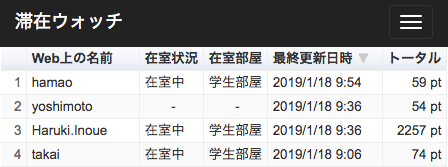
\includegraphics[width=150mm]{image/ListOccupancy.png}
    \caption{在室情報のリスト}
    \label{fig:list}
  \end{center}
\end{figure}

\begin{figure}[H]
  \begin{center}
    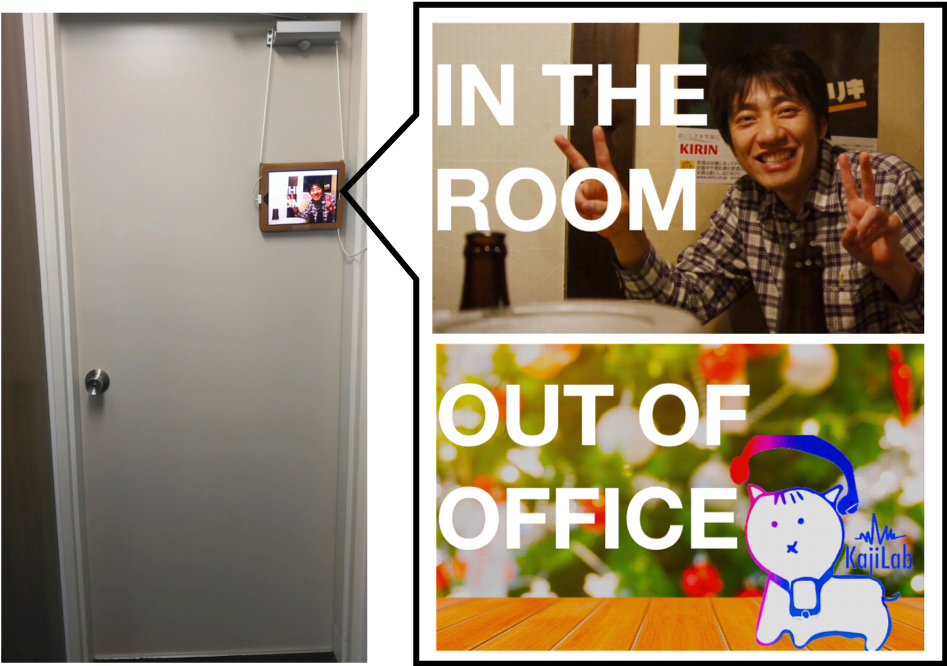
\includegraphics[width=150mm]{image/OccupancyMonitor.png}
    \caption{教員の在室状況モニタ}
    \label{fig:monitor}
  \end{center}
\end{figure}

過去の在室状況からは利用者が人の訪問場所の傾向が把握できるため,次の人の訪問場所の予測がある程度可能である.
これにより,円滑なコミュニケーションの補助になると考える.
例えば,相手に会う約束をするほどではないが,一緒に作業をしたら効率が良くなるといった場合が該当する.
管理者は部屋の利用状況を把握でき,室内の温度調整を始めとする環境整備や活用状況が少ない部屋の省エネ化の指標となる.
そこで過去の在室履歴を図\ref{fig:staytime}の滞在時間,図\ref{fig:weekday}の曜日別の滞在率,図\ref{fig:group}の班別の滞在率,図\ref{fig:total}の合計滞在時間をグラフで示している.

% \begin{figure}[H]
%   \begin{center}
%     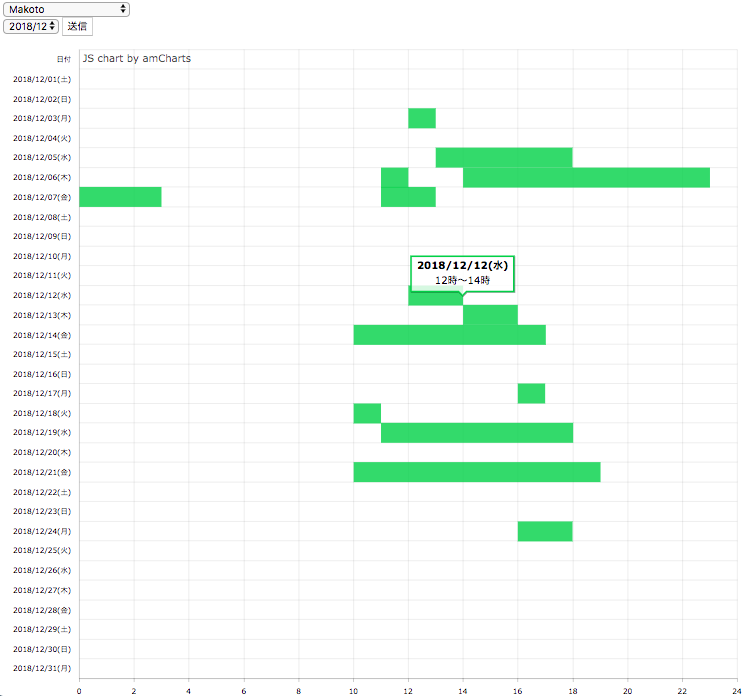
\includegraphics[width=160mm]{image/StayTime.png}
%     \caption{滞在時間のグラフ}
%     \label{fig:staytime}
%   \end{center}
% \end{figure}

% \begin{figure}[H]
%   \begin{center}
%     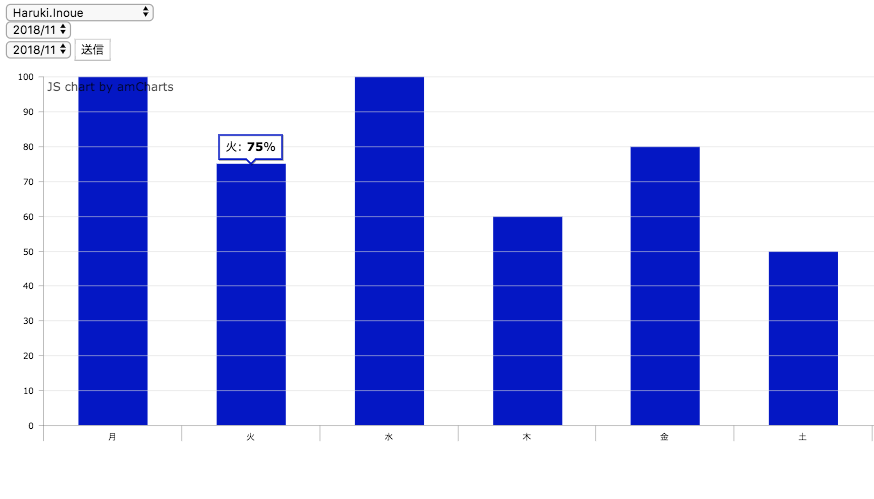
\includegraphics[width=160mm]{image/StayRateWeek.png}
%     \caption{曜日別の滞在率のグラフ}
%     \label{fig:weekday}
%   \end{center}
% \end{figure}

% \begin{figure}[H]
%   \begin{center}
%     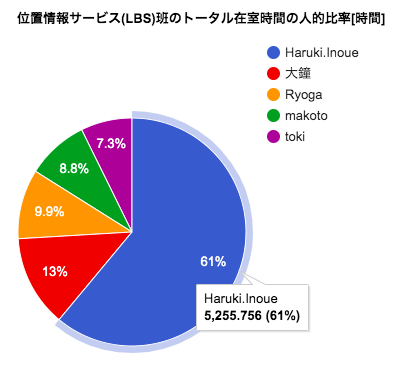
\includegraphics[width=150mm]{image/StayRateGroup.png}
%     \caption{班別の滞在率のグラフ}
%     \label{fig:group}
%   \end{center}
% \end{figure}

% \begin{figure}[H]
%   \begin{center}
%     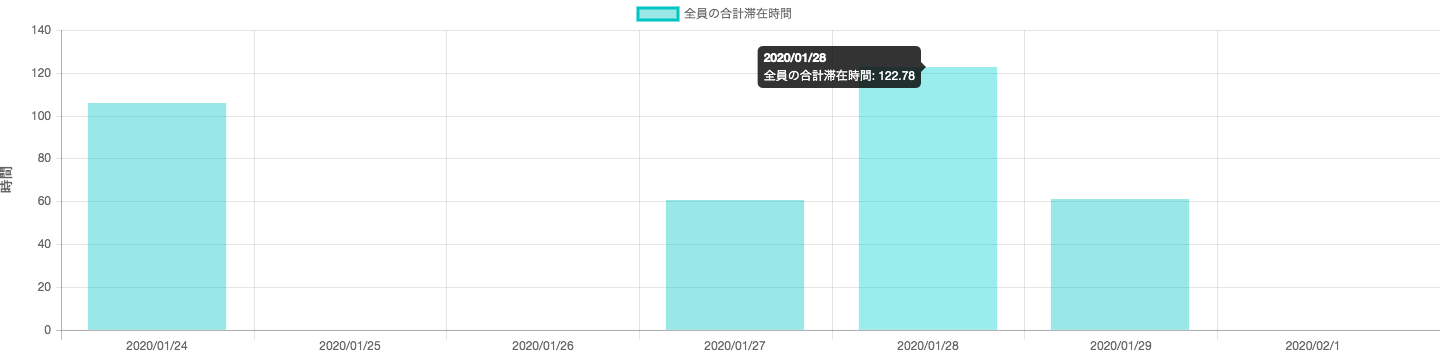
\includegraphics[width=160mm]{image/TotalStayTime.png}
%     \caption{合計滞在時間のグラフ}
%     \label{fig:total}
%   \end{center}
% \end{figure}




